\documentclass[aspectratio=169,9pt]{beamer}
\usetheme{default}
\usepackage[T1]{fontenc}
\usepackage[default]{sourcesanspro}
\usepackage{tikz}
\usetikzlibrary{arrows.meta}

\definecolor{accent}{HTML}{2F74C0}
\definecolor{ink}{HTML}{1C2733}
\definecolor{muted}{HTML}{5A6A7C}
\definecolor{paper}{HTML}{EEF3F8}

\setbeamertemplate{navigation symbols}{}
\setbeamercolor{normal text}{fg=ink}
\setbeamercolor{frametitle}{fg=accent}
\setbeamerfont{frametitle}{series=\bfseries,size=\large}
\setbeamertemplate{itemize item}{\color{accent}\raisebox{0.2em}{\scalebox{0.55}{$\blacksquare$}}}
\setbeamertemplate{frametitle}{%
  \vspace{0.9em}\insertframetitle\par\vspace{0.2em}{\color{accent}\rule{\textwidth}{0.5pt}}%
  \begin{tikzpicture}[remember picture, overlay]
    \node[anchor=north east, inner sep=0] at ([xshift=-0.9em, yshift=-0.5em]current page.north east)
      {\includegraphics[height=2.2em]{../../book/logo.png}};
  \end{tikzpicture}}
\setbeamertemplate{footline}{\hspace{1.2em}{\color{muted}\tiny antadatabase.com \quad Antoine Hermant, University of Bern}\hfill{\color{muted}\tiny\insertframenumber\,/\,\inserttotalframenumber}\hspace{1.2em}\vspace{0.7em}}
\setlength{\leftmargini}{0.9em}

% A box with a title, for the columns of slide 2
\newcommand{\panel}[2]{%
  \begin{tikzpicture}
    \node[fill=paper, rounded corners=3pt, inner sep=6pt, text width=\linewidth-12pt, anchor=north west] {%
      \begin{minipage}[t][14.6em][t]{\linewidth}\footnotesize
      {\color{accent}\bfseries\small #1}\par\vspace{0.5em}#2
      \end{minipage}};
  \end{tikzpicture}}
\newcommand{\hl}[1]{{\color{accent}\bfseries #1}}

\begin{document}

% ---------------------------------------------------------------- slide 1
\begin{frame}
\frametitle{AntADatabase: the radar isochrones of Antarctica in one place}
\begin{columns}[T]
\begin{column}{0.36\textwidth}
\textbf{Purpose:} gather every published radar isochrone (IRH) of the Antarctic ice sheet, with its age, in one format, to constrain ice-sheet models.

\vspace{1em}
\textbf{v1, online since November 2026}\par\vspace{0.4em}
\begin{tabular}{@{}r@{\hspace{0.6em}}l@{}}
\hl{18}     & datasets \\
\hl{1,014}  & radar lines \\
\hl{160}    & dated isochrones \\
\hl{248 MB} & netCDF, on the cloud
\end{tabular}

\vspace{1em}
\begin{itemize}\setlength{\itemsep}{0.4em}
\item \textbf{3D viewer} in the browser
\item \textbf{Python package}: sync, then query by age, region or dataset
\item \textbf{Submission portal}: automatic checks and a private 3D preview
\end{itemize}
\end{column}
\begin{column}{0.6\textwidth}
\vspace{0.3em}
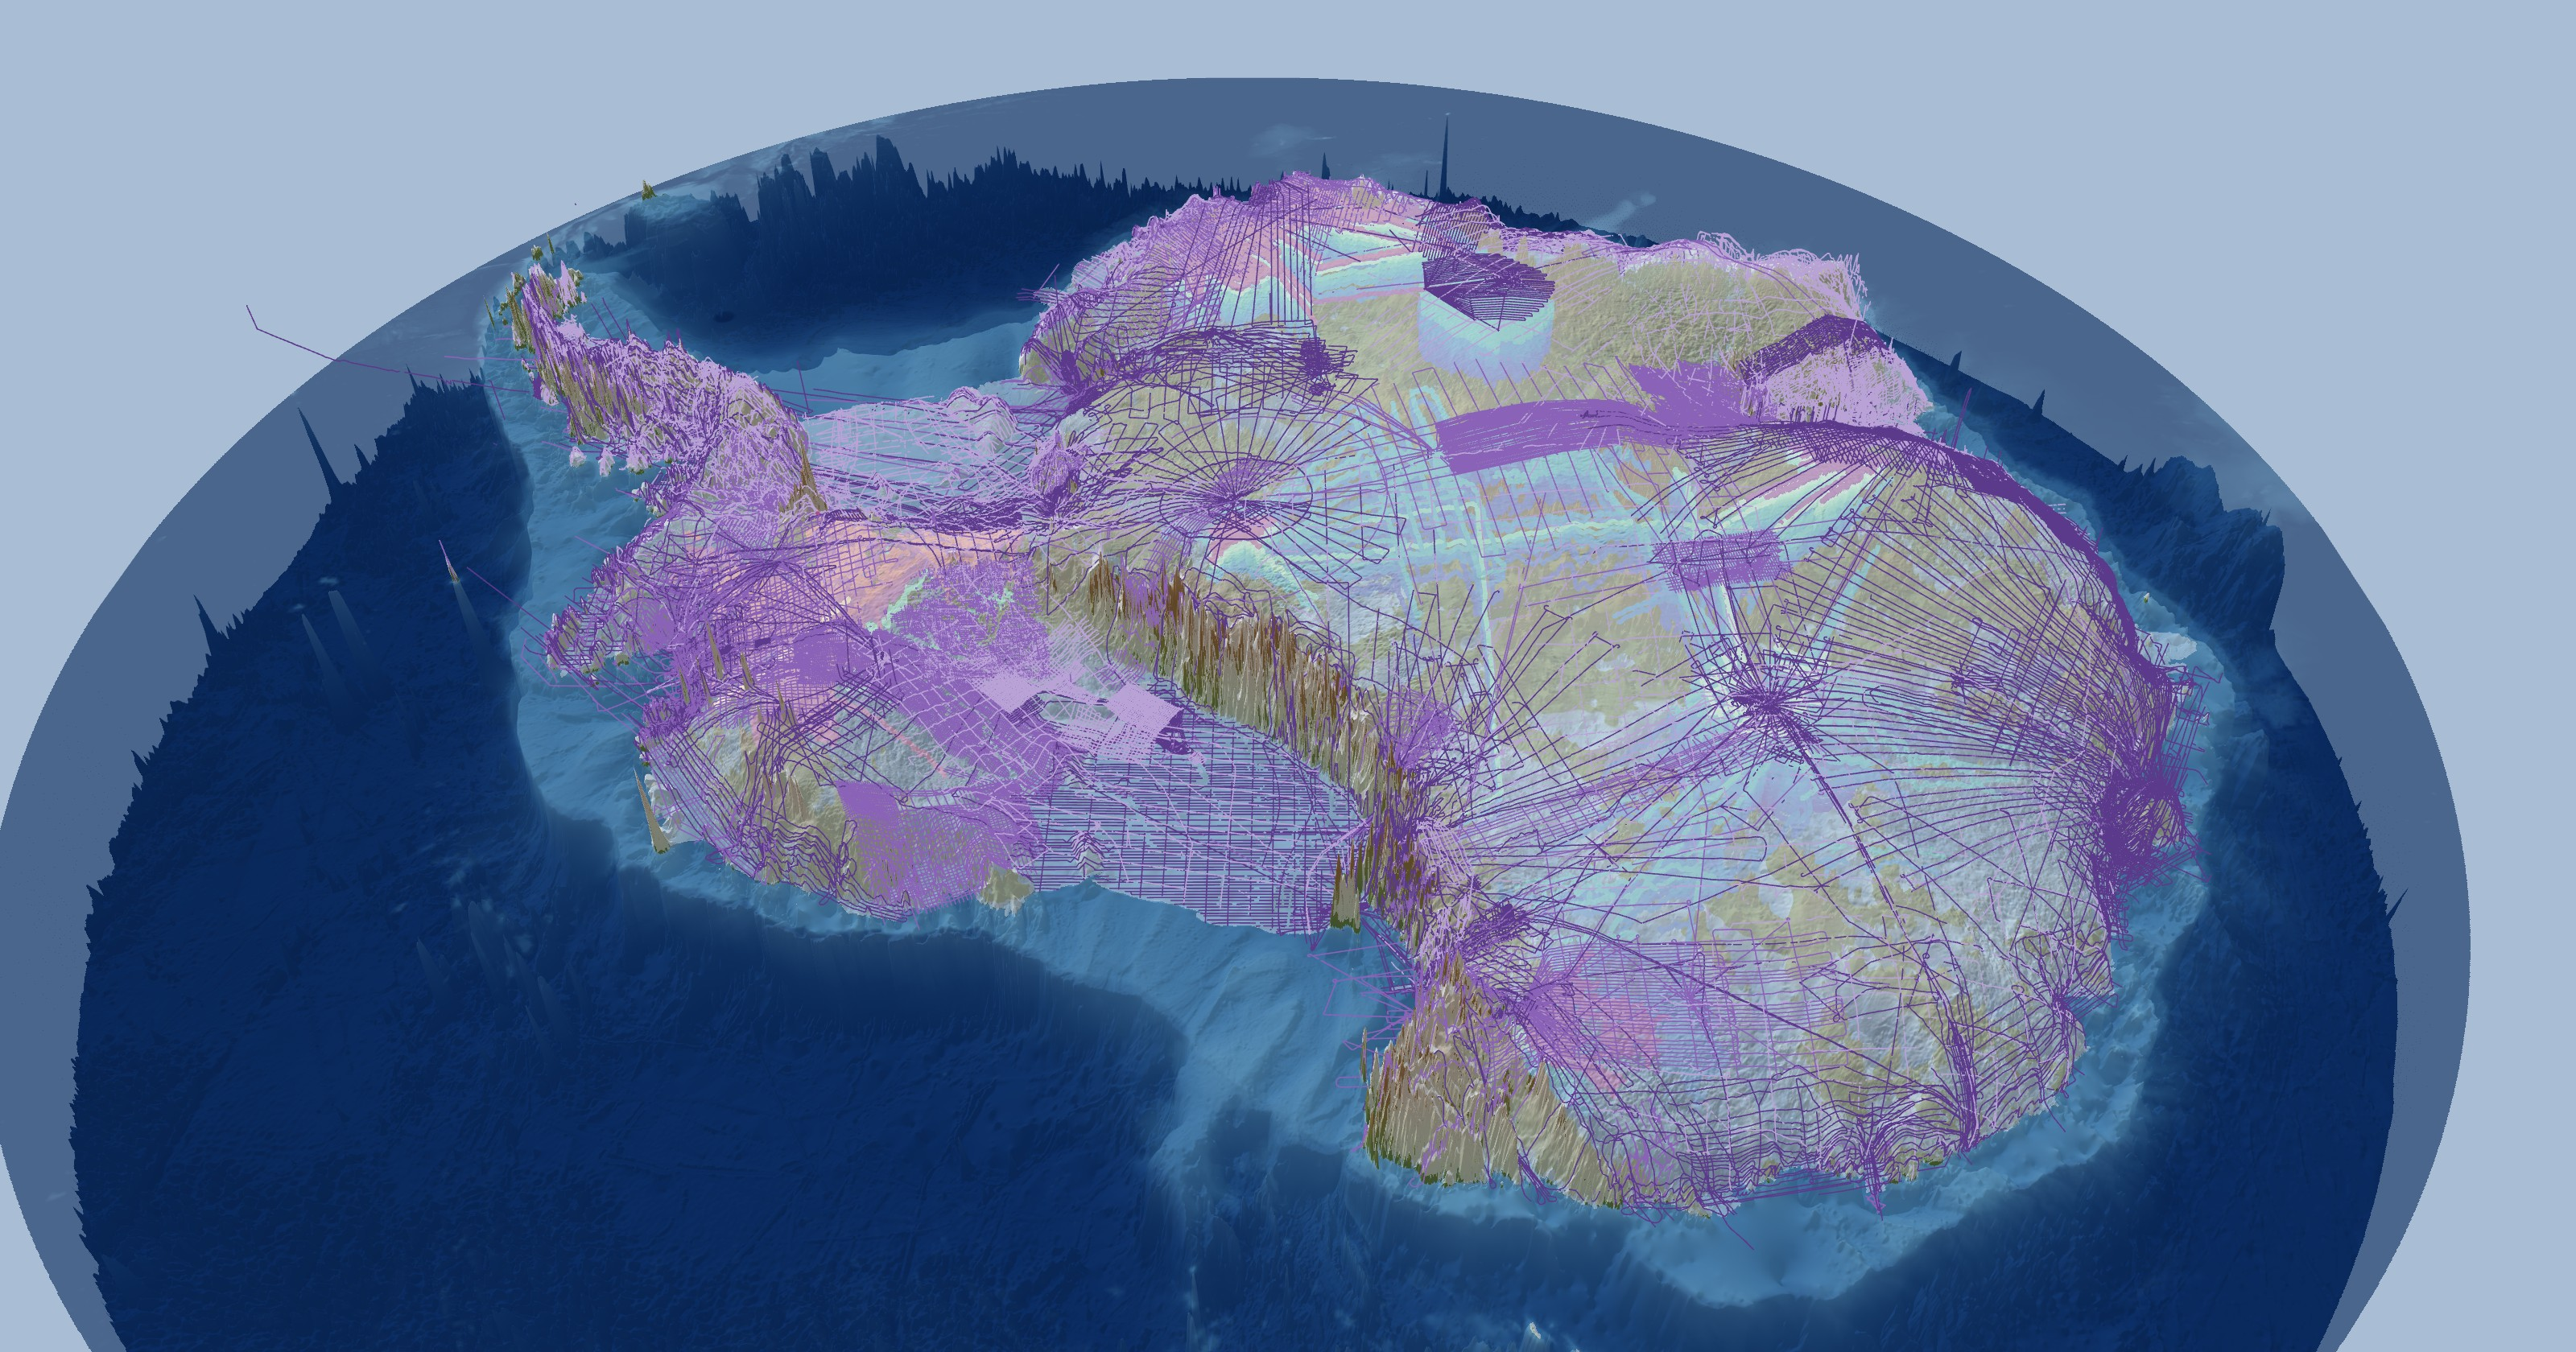
\includegraphics[width=\linewidth]{viewer-bedmap.jpg}\par
{\tiny\color{muted} The 3D viewer: the isochrones under the ice surface, and in purple the Bedmap 1--3 radar survey lines, most of them not traced yet. antadatabase.com/viewer}
\end{column}
\end{columns}
\end{frame}

% ---------------------------------------------------------------- slide 2
\begin{frame}
\frametitle{Towards v2: a consistent, harmonised database, ready for ML}
\vspace{0.3em}
\begin{columns}[T]
\begin{column}{0.325\textwidth}
\panel{1.\; v2, from the raw files}{%
\begin{itemize}\setlength{\itemsep}{0.35em}
\item \textbf{Uniform metadata}: dating method, ice core, chronology and firn correction of every layer
\item \textbf{Checked}: layers below the bed, crossing layers, spikes
\item \textbf{Reconnected to Bedmap 1--3}: the same radar traces fill the missing ice thickness, bed and surface (median difference \hl{$<$\,1\,m})
\end{itemize}}
\end{column}
\begin{column}{0.325\textwidth}
\panel{2.\; Harmonising the layers}{%
\begin{itemize}\setlength{\itemsep}{0.35em}
\item \textbf{Network}: \hl{18,500\,km} of shared tracks and 1,674 crossings between datasets; 9 ice cores on the lines
\item \textbf{Match} the same layer across datasets $\rightarrow$ \emph{horizons}
\item \textbf{Date} them at the cores, with the latest chronologies
\item Published ages kept, harmonised ages added
\end{itemize}}
\end{column}
\begin{column}{0.325\textwidth}
\panel{3.\; Files for models and ML}{%
\begin{itemize}\setlength{\itemsep}{0.35em}
\item \textbf{Line view}: one netCDF per dataset
\item \textbf{Layer view}: one netCDF per horizon, a whole layer in one read
\item \textbf{Parquet} on the cloud: training pipelines read only the rows they need, straight from the bucket
\item \textbf{One index} to query by horizon, age, region or core
\item Designed with \textbf{US colleagues in Texas}, for training ML models on the cloud
\end{itemize}}
\end{column}
\end{columns}

\vspace{0.8em}
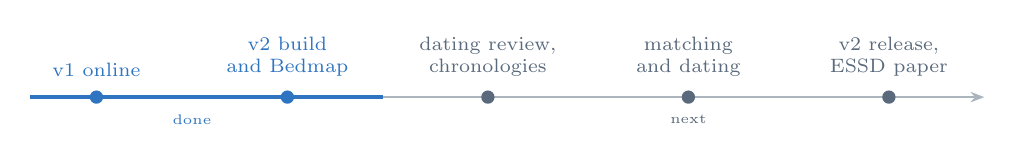
\begin{tikzpicture}[x=\textwidth/5, every node/.style={font=\scriptsize, align=center}]
  \draw[muted!50, line width=1pt, -{Stealth[length=5pt]}] (0,0) -- (5,0);
  \draw[accent, line width=1.4pt] (0,0) -- (1.85,0);
  \foreach \x/\t/\c in {0.35/{v1 online}/accent, 1.35/{v2 build\\and Bedmap}/accent, 2.4/{dating review,\\chronologies}/muted, 3.45/{matching\\and dating}/muted, 4.5/{v2 release,\\ESSD paper}/muted}{
    \fill[\c] (\x,0) circle (2.4pt);
    \node[above=4pt, text=\c] at (\x,0) {\t};
  }
  \node[below=3pt, text=accent, font=\tiny] at (0.85,0) {done};
  \node[below=3pt, text=muted, font=\tiny] at (3.45,0) {next};
\end{tikzpicture}
\end{frame}

\end{document}
